

\chapter{Results}

In this chapter, we present approaches for attacking machine learning algorithms with adversarial techniques presented in the previous chapter. We discuss that the knowledge of the architecture and weight parameters is sufficient to derive adversarial samples against DNNs. Further discussion goes into black box attacks where the attack has minimal information about the underlying system. The discussion is then closed with how model's knowledge can be transferred between different algorithms/techniques.

\section{Fully balanced model}

Recall that the object of this research is to understand the effects of adversarial attacks on imbalanced CNNs. However, it is firstly required to create the baseline for our comparisons. This consists of creating perturbation on every class label and querying its accuracy on a fully balanced model. Canonical models assume that every object in the dataset are sampled from similar distributions. However, in real-life situations, even though the number of samples is the same, some class labels could be poorly represented by the lack of a clear structure. This could often lead to differences in the output for each specific class \cite{krawczyk2016learning}. On this way, dataset balance by itself does not guarantee that the model will equally generalise across all classes.
\begin{figure}[H]
	\centering
	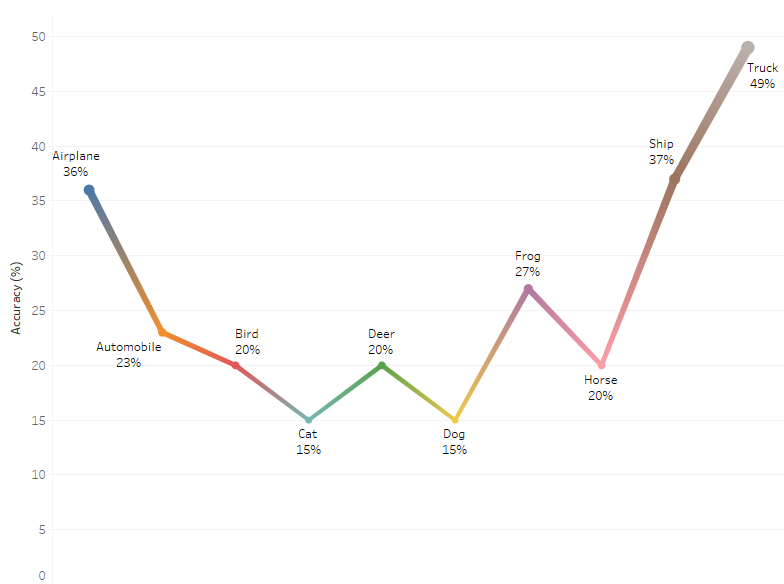
\includegraphics[scale=0.7]{balanced_perturbed.png}
	\caption{Individual class accuracy on the balanced model}
	\label{fig:balanced_perturbed}
\end{figure}

Figure ~\ref{fig:balanced_perturbed} shows that the accuracy for all classes is drastically reduced when the balanced model is presented with adversarial examples. Even though there is enough samples for each class, the adversarial attack forces the domain shift of each individual sample towards different regions in space, causing a misclassification of the current label. The effectiveness of the adversarial attack can be partially explained by the balancing of the dataset itself. In a model where the dataset used in training aims for normalization over all classes, the network is often caught in trying to find weights and biases that generalizes well over all set of labels. Therefore, perturbations become more efficient due to a bigger proximity of classes distributions in space.


\section{Class undersampling and oversampling}

As the number of samples on a target class goes down, an increase of vulnerability towards that specific label is expected when compared to the balanced model. However, the results on table  ~\ref{tbl:results} shows the opposite. The network capacity to learn is often confused with the amount of samples for each class and it does not take into consideration the overlap of different class distributions over space.

The adversarial test shows this results from two perspectives. Firstly, on the class undersampling the accuracy for each individual class was on average above 50\%, which already demonstrates better robustness when compared to the balanced case. This could be explained by having the data distribution of that specific class being squished into space and, hence, reducing the size of its vicinity with other classes. Therefore, the degree of the perturbation is reduced since the class gradient has lower influence on the overall gradient. Secondly, when oversampling occurs, it is expected to have the target class expanding into space and taking as much space as possible when compared to other classes. This happens since the network performs more gradient updates on that specific class due to the amount of available samples. Perturbation on this case had very low effect, as the small push cause by our $\epsilon$ was not enough to move points to outside of their distributions.
\begin{table}[H]
	\centering
	
	\begin{tabular}{lcccccc}
		\toprule
		&\multicolumn{2}{c}{Balanced}
		&\multicolumn{2}{c}{Undersampling}
		&\multicolumn{2}{c}{Oversampling} 
		\\\cmidrule(r){2-3}\cmidrule(l){4-5}\cmidrule(l){6-7}
		Class Label &Non-Pert. &Pert. &Non-Pert. &Pert. &Non-Pert. &Pert.      \\
		\midrule
		0 - Airplane &84\%& 36\% &69\%& 19\%    & 89\% &87\%      \\
		1 - Automobile &88\%& 23\% &77\%& 16\%    & 93\% &91\%      \\
		2 - Bird &80\%& 20\% &48\%& 9.4\%    & 79\% &73\%      \\
		3 - Cat &69\%& 11\% &26\%& 0.5\%    & 76\% &72\%      \\
		4 - Deer &85\%& 20\% &70\%& 9.8\%    & 85\% &80\%      \\
		5 - Dog &77\%& 15\% &58\%& 9\%    & 80\% &76\%      \\
		6 - Frog &88\%& 27\% &83\%& 20\%    & 89\% &88\%      \\
		7 - Horse &83\%& 20\% &69\%& 18\%    & 90\% &88\%      \\
		8 - Ship &90\%& 37\% &80\%& 19\%    & 92\% &89\%      \\
		9 - Truck &93\%& 49\% &80\%& 21\%    & 91\% &87\%      \\
		\bottomrule
	\end{tabular}
	\caption{Results for the undersampling and oversampling models}
	\label{tbl:results}
\end{table}

\section{Overlapping distributions}
When objects in the dataset already have distributions that are very clear to one another the effects of adversarial seems to be stronger. Figure ~\ref{fig:conf_matrix_full} shows that for the pairs Cat/Dog and Automobile/Truck, misclassification naturally happens towards one another due to similarities in their feature space \cite{stanford2016}. On this case, our experiment shows that the adversarial attack intensifies the property by increasing the number on which one class is picked over another. This property gives interesting insights, as it shows that the gradient sign is really navigating around the target class distribution and when a overlap occurs it becomes easier to create an adversarial.

\begin{figure}[ht] 
	\label{fig7} 
	\begin{minipage}[b]{0.5\linewidth}
		\centering
		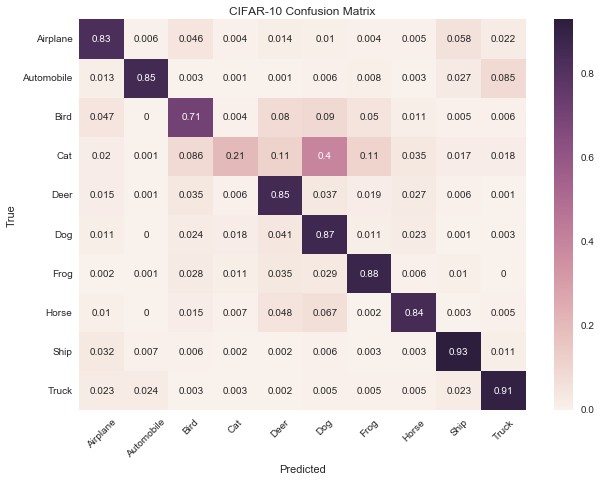
\includegraphics[width=1\linewidth]{cat_undersampling_per.png} 
		\vspace{4ex}
	\end{minipage}%%
	\begin{minipage}[b]{0.5\linewidth}
		\centering
		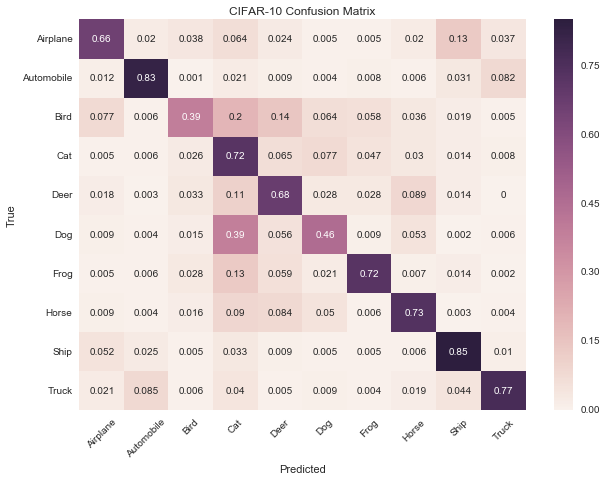
\includegraphics[width=1\linewidth]{cat_oversampling_per.png} 
		\vspace{4ex}
	\end{minipage} 
	\begin{minipage}[b]{0.5\linewidth}
		\centering
		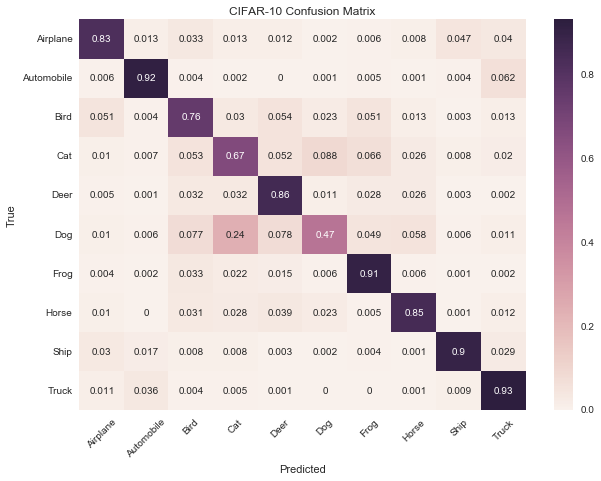
\includegraphics[width=1\linewidth]{dog_undersampling_per.png} 
		\vspace{4ex}
	\end{minipage}%% 
	\begin{minipage}[b]{0.5\linewidth}
		\centering
		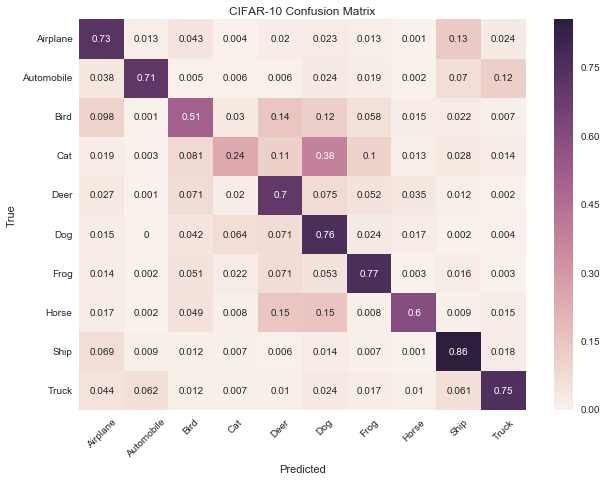
\includegraphics[width=1\linewidth]{dog_oversampling_per.png} 
		\vspace{4ex}
	\end{minipage} 
	\centering
	\caption{Top Left and Right: Cat undersampling / oversampling with perturbation. Bottom Left and Right: Dog undersampling / oversampling with perturbation}
\end{figure}